\documentclass{article}
\usepackage[T1]{fontenc}
\usepackage{lmodern}
\usepackage{graphicx}
\usepackage{amsmath,amssymb}
\usepackage[a4paper,margin=2cm]{geometry}
\usepackage[absolute,overlay]{textpos}
\setlength{\TPHorizModule}{1mm}
\setlength{\TPVertModule}{1mm}
\usepackage[indonesian]{babel}
\usepackage{hyperref}
\setlength{\emergencystretch}{2em}
% unit: Halaman 62

\begin{document}

% === Halaman 62 (llm) ===

\vspace{40mm}

$f(K_i, P)$ dinamakan fungsi putaran, $r$ adalah jumlah putaran

\textbf{DES: $r = 16$}\
\textbf{AES-128/192/256: $r = 10/12/14$}

% deskripsi: Diagram blok proses enkripsi dengan pembuatan sub-key (Sub-key generation) yang memberikan kunci $K_1, K_2, K_3, \dots, K_r$ ke dalam serangkaian fungsi putaran $f$ yang memproses input $P$ menjadi output $C$.
% bbox normalisasi: [0.1500, 0.0900, 0.9300, 0.6500]
\begin{textblock*}{163.80mm}(31.50mm,26.73mm)
\noindent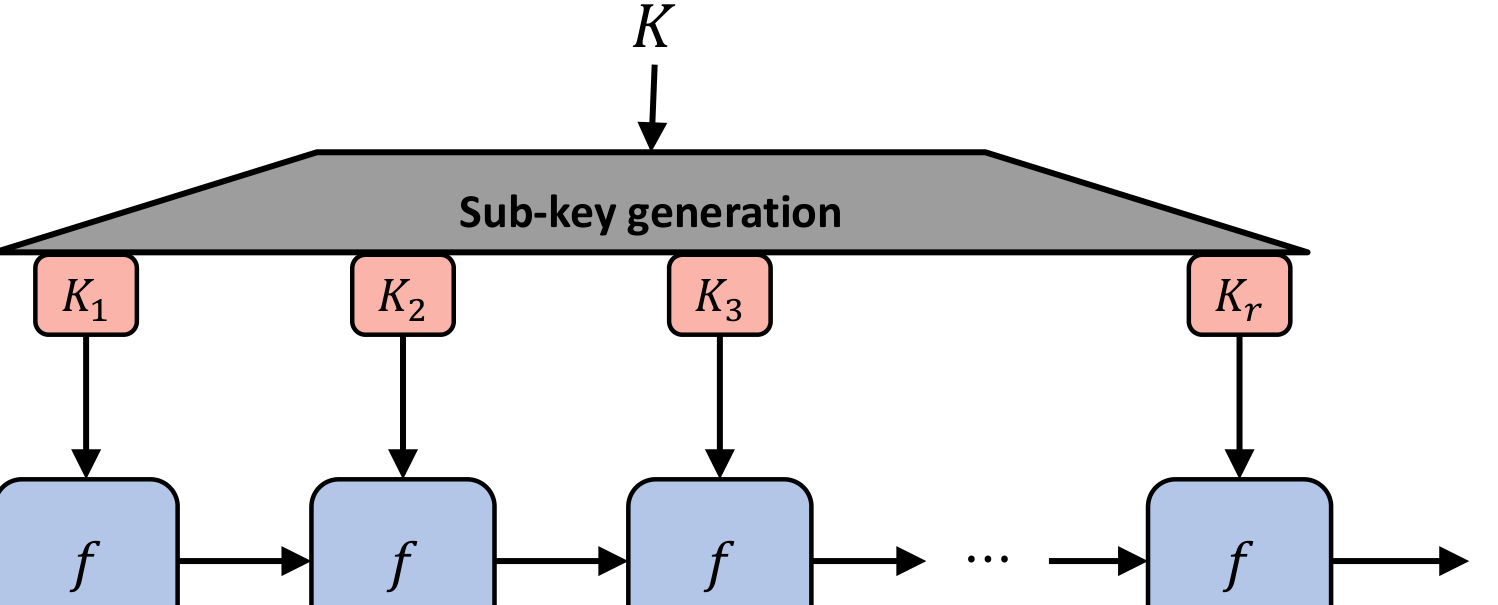
\includegraphics[width=163.80mm,height=166.32mm]{../../images/llm/page_062_img_01.png}%
\end{textblock*}

\end{document}
